%% Version 5.0, 2 January 2020
%
%%%%%%%%%%%%%%%%%%%%%%%%%%%%%%%%%%%%%%%%%%%%%%%%%%%%%%%%%%%%%%%%%%%%%%
% TemplateV5.tex --  LaTeX-based template for submissions to the 
% American Meteorological Society
%
%%%%%%%%%%%%%%%%%%%%%%%%%%%%%%%%%%%%%%%%%%%%%%%%%%%%%%%%%%%%%%%%%%%%%
% PREAMBLE
%%%%%%%%%%%%%%%%%%%%%%%%%%%%%%%%%%%%%%%%%%%%%%%%%%%%%%%%%%%%%%%%%%%%%

%% Start with one of the following:
% DOUBLE-SPACED VERSION FOR SUBMISSION TO THE AMS
\documentclass{ametsocV5}

% TWO-COLUMN JOURNAL PAGE LAYOUT---FOR AUTHOR USE ONLY
% \documentclass[twocol]{ametsocV5}


% Enter packages here. If too many math alphabets are used,
% remove unnecessary packages or define hmmax and bmmax as necessary.

%\newcommand{\hmmax}{0}
%\newcommand{\bmmax}{0}
\usepackage{amsmath,amsfonts,amssymb,bm}
\usepackage{mathptmx}%{times}
\usepackage{newtxtext}
\usepackage{newtxmath}
\usepackage{natbib}


%%%%%%%%%%%%%%%%%%%%%%%%%%%%%%%%

%%% To be entered by author:

%% May use \\ to break lines in title:

\title{Quantifying Uncertainty in Forecast-Based Anticipatory Action Triggers Using Bootstrapping Methods}

%%% Enter authors' names, as you see in this example:
%%% Use \correspondingauthor{} and \thanks{Current Affiliation:...}
%%% immediately following the appropriate author.
%%%
%%% Note that the \correspondingauthor{} command is NECESSARY.
%%% The \thanks{} commands are OPTIONAL.

    %\authors{Author One\correspondingauthor{Author name, email address}
% and Author Two\thanks{Current affiliation: American Meteorological Society, 
    % Boston, Massachusetts.}}

\author{%
Max Mauerman\affmark[1]\correspondingauthor{Max Mauerman, max.mauerman@columbia.edu}, Kevin Schwarzwald\affmark[1], Daniel Osgood\affmark[1], Nathan Lenssen\affmark[2], and Abdel-Lathif Younous\affmark[3]\\
\affaddr{\affmark[1] Columbia University Climate School}\\
\affaddr{\affmark[2] Colorado School of Mines \& NSF National Center for Atmospheric Research}\\
\affaddr{\affmark[3] United Nations World Food Programme}\\
}

%%%%%%%%%%%%%%%%%%%%%%%%%%%%%%%%%%%%%%%%%%%%%%%%%%%%%%%%%%%%%%%%%%%%%
% ABSTRACT
%
% Enter your abstract here
% Abstracts should not exceed 250 words in length!
%
 

\abstract{As of 2022, nearly 5 million smallholder farmers across a dozen countries are covered by Anticipatory Action (AA) programs \citep{chaves-gonzalez_anticipatory_2022}, which are aid schemes triggered if seasonal forecasts of rainfall cross a locally-determined threshold. AA thresholds are often calculated to meet a donor- or government-specified expected trigger frequency \citep{coughlan_de_perez_adapting_2022,world_food_programme_10_2024}. However, the observational rainfall record in many regions with AA programs is limited, and interannual and interdecadal autocorrelation in the climate patterns driving seasonal rainfall further reduce the effective sample size used to calculate these thresholds \citep{martinez_seasonal_2022}. Thus, AA triggers are highly sensitive to the limited observational record, increasing the risk that action is not triggered when it is needed or that programs become financially unsustainable due to excessive triggers. In practice, forecasters are aware of this uncertainty, and ad hoc decisions on whether to trigger action are often made if seasonal forecasts are close to the threshold. Seeking a more formalized, statistically sound alternative to ad hoc approaches, governments and humanitarian agencies have asked for transparent and intuitive metrics for forecast trigger uncertainty. To address this demand, we develop a method for quantifying the uncertainty in thresholds due to a limited observational record using bootstrap resampling. Examining United Nations operational AA forecasts in sub-Saharan Africa, we demonstrate how our method provides a better quantification of critical underlying uncertainty, enabling these AA systems to meet the state-of-the-art demanded by donors and the WMO.}
\begin{document}

%% Necessary!
\maketitle

%%%%%%%%%%%%%%%%%%%%%%%%%%%%%%%%%%%%%%%%%%%%%%%%%%%%%%%%%%%%%%%%%%%%%
% SIGNIFICANCE STATEMENT/CAPSULE SUMMARY
%%%%%%%%%%%%%%%%%%%%%%%%%%%%%%%%%%%%%%%%%%%%%%%%%%%%%%%%%%%%%%%%%%%%%
%
% If you are including an optional significance statement for a journal article or a required capsule summary for BAMS 
% (see www.ametsoc.org/ams/index.cfm/publications/authors/journal-and-bams-authors/formatting-and-manuscript-components for details), 
% please apply the necessary command as shown below:
%
% \statement
% Significance statement here.
%
% \capsule
% Capsule summary here.


%%%%%%%%%%%%%%%%%%%%%%%%%%%%%%%%%%%%%%%%%%%%%%%%%%%%%%%%%%%%%%%%%%%%%
% MAIN BODY OF PAPER
%%%%%%%%%%%%%%%%%%%%%%%%%%%%%%%%%%%%%%%%%%%%%%%%%%%%%%%%%%%%%%%%%%%%%
%

%% In all cases, if there is only one entry of this type within
%% the higher level heading, use the star form: 
%%
% \section{Section title}
% \subsection*{subsection}
% text...
% \section{Section title}

%vs

% \section{Section title}
% \subsection{subsection one}
% text...
% \subsection{subsection two}
% \section{Section title}

%%%
% \section{First primary heading}

% \subsection{First secondary heading}

% \subsubsection{First tertiary heading}

% \paragraph{First quaternary heading}

\section{Introduction}

% Max to draft and Dan to refine. 

Humanitarian agencies are trying to be less reactive... advances in the state of the science on seasonal forecasting make early action against drought feasible... But forecasts need to follow standards of consistency, robustness and transparency a la WMO guidelines, especially when lives are on the line... it is not always obvious how to pragmatically account for uncertainty under those guidelines... our paper advances a simple method for quantifying one type of uncertainty, which is how sensitive the trigger definition is to the limited historical record... this method was developed to respond to practical needs from WFP, and can be replicated elsewhere. 

\section{Forecast-based anticipatory action}

\subsection{Institutional background of AA}

% Abdel to help write this part.

When did the UN start using forecasts for humanitarian action? What about seasonal forecasts in particular? What obstacles (scientific and practical) have kept this from happening sooner? Some parallels to similar problems in the area of parametric insurance. 

\subsection{The PyCPT seasonal forecasting method}

% Max to write but could probably use Kevin and Nathan's eyes to make sure I'm not saying anything scientifically out of pocket.
% Dan style note: "PyCPT" instead of "NextGen" 
% Talk about heuristic rules that the country offices were using, and how they are similar conceptually / functionallty to bootstrapping 

Talk about the types of seasonal forecasts we are using here, where they come from and how to interpret them. Can draw from a lot of prior IRI work here. Key talking points are that NextGen is a method to produce downscaled and bias-corrected seasonal forecasts using a multi-model ensemble of GCMs. The models, predictand and calibration parameters can be customized to each locality and context. Local met services use the method and software to create purpose-built forecast models for their country or region. Forecasts are presented as the probability of non-exceedance at a given percentile threshold (not only terciles).

\subsection{Triggering humanitarian action using seasonal forecasts}

% Max to write with Abdel's input.

Talk about the mechanics of how we define a forecast action trigger here. Below is how I wrote it up for WFP in Ethiopia: 

A core component of the Anticipatory Action Plan is the forecast “trigger”, i.e., the quantitative threshold of predictive certainty above which a certain anticipatory action will be taken. 
This document describes the procedure used to determine triggers for the WFP AA project and the rationale for why it was implemented this way. At the end of this document, there are links to a set of live documents which provide the most up to date trigger information for each active region and woreda in the AA project.

The basic rationale behind the choice of triggers is that they should be transparent, consistently applied and easily related to the expected frequency with which action will be taken. A humanitarian agency planning budgets for AA programs should be able to look at the trigger rule associated with a specific action and know that it is likely to occur - for example - 20 percent  of the time, based on historical analysis. 

Accordingly, the trigger rule used for this AAP is based on a consistent frequency of action for a given type of programming, across locations and times of year. For instance, in Somali Region, “Severe” level actions are associated with a 20 percent frequency of action. This means that for a given location, for the forecast issued in a given month, we should expect Severe actions to trigger during the strongest 20pct of drought forecasts. To determine the numeric threshold associated with acting 20pct of the time, we rank all of the historical forecasts (“hindcasts”) available from the least likely prediction of drought to the most likely, and compute the 20th percentile of this distribution.

Talk a little about the sensitivity of this method to the choice of threshold, and what to do when the forecast is just a couple pp above or below the threshold. This is something that practitioners always have to deal with, and they have heuristic ways of managing it, but those can be inconsistent. We propose here a more systematic solution... segues into discussion about sources of uncertainty.

\section{Sources of forecast uncertainty}

% Nathan - can fold most of this into section 2b, since it isn't really a standalone section 

% Kevin to write w Max and Nathan as needed.
% The basic strategy is to go through all of the different commonly discussed sources of uncertainty, and talk about how they are addressed in the NextGen approach, except for the problem of the limited historical record. That is what we're addressing with this paper. 

% note Aug 13: Can pare down the discussion of the first four sources of uncertainty, since they aren't the main point. 

\subsection{Uncertainty in modeling choices}

Different GCMs have different assumptions about how things work. We account for this by using a multi-model ensemble in predictions.

\subsection{Uncertainty in initial conditions}

I'm not sure if or how to talk about this -- I'm mostly familiar with this in the context of long-term climate change projections, not seasonal forecasting. As I understand it, all of the GCM output that we use for seasonal forecasting is initialized with the same conditions for a given issue month. So maybe this is not a huge issue the way it is for CC projections, where uncertainty in initial conditions can propagate further (cf Schwarzwald and Lenssen 2022). But maybe I'm also missing something, so it would be good to get your input. 

In any case, we can talk about how we use forecasts at different lead times, with the decision rule putting greater weight on forecasts with a shorter lead time, since we are more certain about the initial conditions.

\subsection{Uncertainty in accuracy of predictions}

The bias correction and calibration components of NextGen are meant to account for this. I need to bug Andy R. and Azhar about this since they have promised a more thorough writeup. Talk about the sharpness ratio of quantifying the confidence of the forecast (this is something that decision-makers should also be thinking about, and not only whether the forecast is above or below the threshold).

Note that this section is mostly focusing on how well forecasts predict observed rainfall. There is a second-order question about whether forecasted rainfall is related to humanitarian impacts of drought (e.g. hunger, loss of animals), which is of practical importance to the projects, but not really what this paper is about. We may want to at least mention it in passing. 

\subsection{Uncertainty due to the limited historical record}

What we wrote for the abstract: The observational rainfall record in many regions with AA programs is limited, and interannual and interdecadal autocorrelation in the climate patterns driving seasonal rainfall further reduce the effective sample size used to calculate these thresholds \citep{martinez_seasonal_2022}. Thus, AA triggers are highly sensitive to the limited observational record, increasing the risk that action is not triggered when it is needed or that programs become financially unsustainable due to excessive triggers. In practice, forecasters are aware of this uncertainty, and ad hoc decisions on whether to trigger action are often made if seasonal forecasts are close to the threshold. Seeking a more formalized, statistically sound alternative to ad hoc approaches, governments and humanitarian agencies have asked for transparent and intuitive metrics for forecast trigger uncertainty.

\section{The bootstrapping method for limited data}

% Nathan to write w Kevin and Max and needed

% MAX TODO: Make sure we are using block randomization, with consecutive years. This could help deal with the autocorrelation problem. There is a literature we can tie this to 

% Abdel is particularly interested in the question of whether interannual correlation and / or trends make the calculation of confidence intervals using this method problematic. i need to put on my stats hat this this one. 

% Note that if we were really doing this properly, I think we would want to do the bootstrap sampling during the step of per-pixel model calibration (which happens in CPT), rather than doing it after the fact with areal average data as we are doing here. But that is a matter for a future paper. We want to at least mention it though I think.

% kevin note: we are thinking about this as applicable to things beyond PyCPT, tho, so dont get too hung up about this 

Below is what I've written about the method for WFP. We need to motivate why we're using the method of bootstrapping and why it's reasonable in this context first.

The AA protocol is based on a binary trigger - if the drought forecast is above a given threshold of confidence, it triggers; if it is below this threshold, it does not.

To test how sensitive the protocol is to the exact threshold values chosen, this section presents an uncertainty analysis. This analysis is based on the method of re-estimating the trigger threshold with years randomly omitted from the historical record. Repeating this procedure many times gives us an estimated distribution of how much the threshold might be expected to vary due to sampling error.

In this case, we run 100 iterations of the re-sampling process. In each iteration, 5 years are randomly omitted from the historical record and then the threshold is re-computed.

The box plots below depict the resulting sensitivity range in the trigger threshold for each issue month and severity level. The actual trigger threshold is shown in red. For reference, the climatological odds (the probability of non-exceedence if we were to guess from historical average conditions, without any forecast information) is shown as the dotted line.

If the current forecast is outside of the sensitivity range, this indicates that we have statistically robust evidence that it is above or below the threshold. If the current forecast falls within the sensitivity range, this indicates that we should interpret the trigger result for the current season with caution.


\section{Application to WFP assistance programs}

\subsection{Results}

% Each of these is an active WFP country, and the forecast is for the primary agricultural season in that country, which varies. Need to mention all that stuff along with the model parmeters in an appendix...

% Need to be sure we are using a definition of the percentile that is consistent with what the API uses! R's may not be the same. make sure we are consistent 

% add table of country results, but dont get too into the weeds on country specifics 

% fig 1: simple obs (NOT forecast) illustration of what we are doing
% fig 2: example using actual WFP data. can just be one area-month-freq. we can put the rest in an appendix. 

% tweak visual so that user focuses on the boxplot, not the clim odds 

% Note: The figures seem to get added to the end instead of in-line. I'm guessing that's how it is in the journal?

% note that this method can acommodate compound / multimonth rules 

\subsubsection{Ethiopia}

\begin{figure}
    \centering
    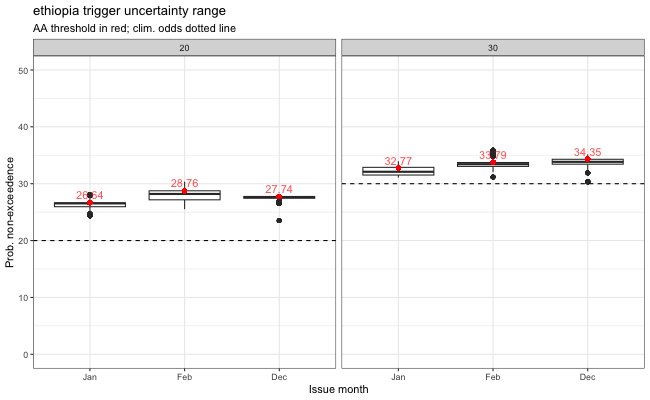
\includegraphics[width=0.9\linewidth]{figures/ethiopia.png}
\end{figure}

\subsubsection{Madagascar}

\begin{figure}
    \centering
    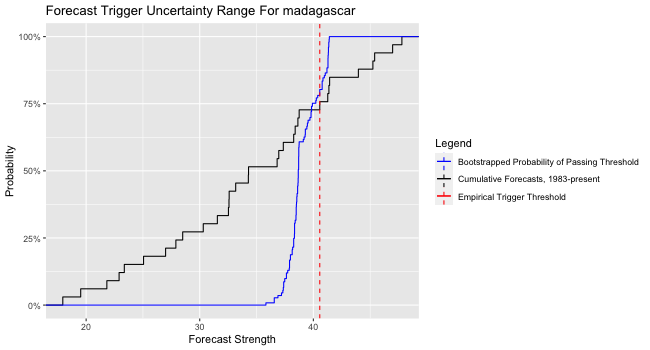
\includegraphics[width=0.9\linewidth]{figures/madagascar.png}
\end{figure}

\subsubsection{Guatemala}

\begin{figure}
    \centering
    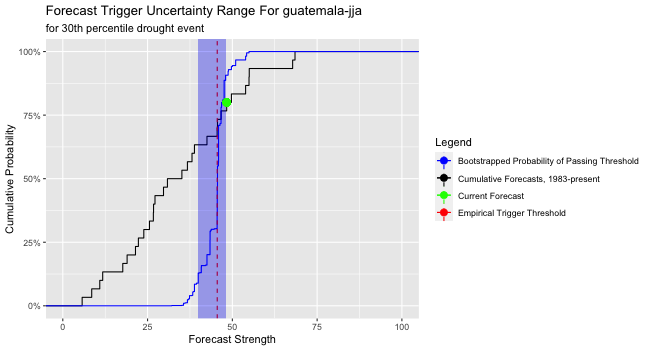
\includegraphics[width=0.9\linewidth]{figures/guatemala-jja.png}
\end{figure}

\subsubsection{Niger}

\begin{figure}
    \centering
    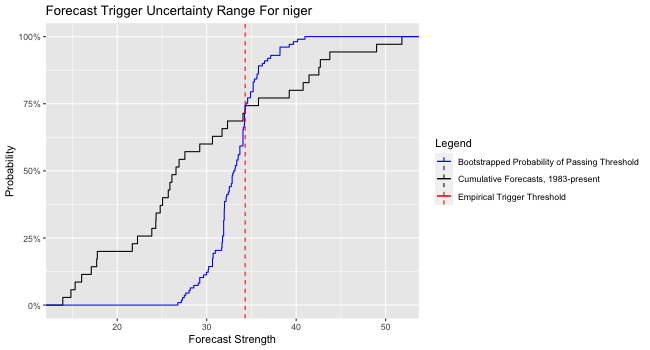
\includegraphics[width=0.9\linewidth]{figures/niger.png}
\end{figure}

\subsubsection{Djibouti}

\begin{figure}
    \centering
    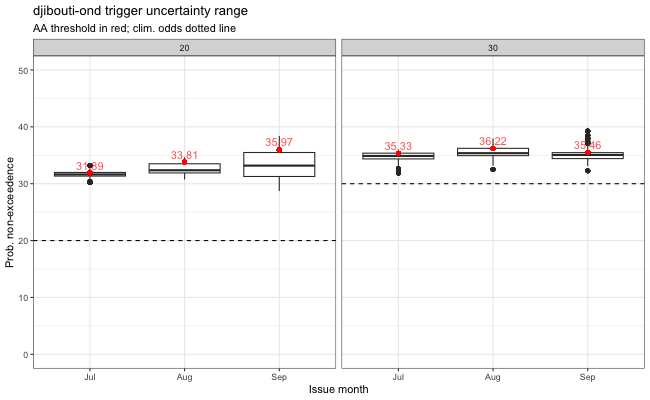
\includegraphics[width=0.9\linewidth]{figures/djibouti-ond.png}
\end{figure}

\subsection{Discussion}

- in general, the range of uncertainty tends to be a couple of percentage points in either direction.
- forecast sharpness generally increases as the lead time decreases, but the threshold uncertainty doesn't.
- likewise, madagascar and guatemala have the sharpest forecasts (which makes some sense; we have reason to think that ENSO teleconnections are relatively stronger there), but have as much or more threshold uncertainy than the other countries.
- this highlights the fact that we have to think about the innate uncertainty from having a short historical record, even in places where we think the forecast model has historically performed well!
- also in some places (ex. Niger) the trigger threshold is statistically indistinguishable from climatological odds. need to be cautious about using the forecast in such places.

% Max to write with Abdel's input.

\section{Conclusions and best practices}

From the abstract:  Examining United Nations operational AA forecasts in sub-Saharan Africa, we demonstrate how our method provides a better quantification of critical underlying uncertainty, enabling these AA systems to meet the state-of-the-art demanded by donors and the WMO.

% Max to draft and Dan to refine.


%%%%%%%%%%%%%%%%%%%%%%%%%%%%%%%%%%%%%%%%%%%%%%%%%%%%%%%%%%%%%%%%%%%%%
% ACKNOWLEDGMENTS
%%%%%%%%%%%%%%%%%%%%%%%%%%%%%%%%%%%%%%%%%%%%%%%%%%%%%%%%%%%%%%%%%%%%%
\acknowledgments
Keep acknowledgments (note correct spelling: no ``e'' between the ``g'' and
``m'') as brief as possible. In general, acknowledge only direct help in
writing or research. Financial support (e.g., grant numbers) for the work
done, for an author, or for the laboratory where the work was performed is
best acknowledged here rather than as footnotes to the title or to an
author's name. Contribution numbers (if the work has been published by the
author's institution or organization) should be included as footnotes on the title page,
not in the acknowledgments.

%%%%%%%%%%%%%%%%%%%%%%%%%%%%%%%%%%%%%%%%%%%%%%%%%%%%%%%%%%%%%%%%%%%%%
% DATA AVAILABILITY STATEMENT
%%%%%%%%%%%%%%%%%%%%%%%%%%%%%%%%%%%%%%%%%%%%%%%%%%%%%%%%%%%%%%%%%%%%%
% 
%
\datastatement
The data availability statement is where authors should describe how the data underlying 
the findings within the article can be accessed and reused. Authors should attempt to 
provide unrestricted access to all data and materials underlying reported findings. 
If data access is restricted, authors must mention this in the statement.

%%%%%%%%%%%%%%%%%%%%%%%%%%%%%%%%%%%%%%%%%%%%%%%%%%%%%%%%%%%%%%%%%%%%%
% APPENDIXES
%%%%%%%%%%%%%%%%%%%%%%%%%%%%%%%%%%%%%%%%%%%%%%%%%%%%%%%%%%%%%%%%%%%%%
%
% Use \appendix if there is only one appendix.
%\appendix

% Use \appendix[A], \appendix[B], if you have multiple appendixes.
%\appendix[A]

%% Appendix title is necessary! For appendix title:
%\appendixtitle{}

%%% Appendix section numbering (note, skip \section and begin with \subsection)
% \subsection{First primary heading}

% \subsubsection{First secondary heading}

% \paragraph{First tertiary heading}

%% Important!
%\appendcaption{<appendix letter and number>}{<caption>} 
%must be used for figures and tables in appendixes, e.g.,
%
%\begin{figure}
%\noindent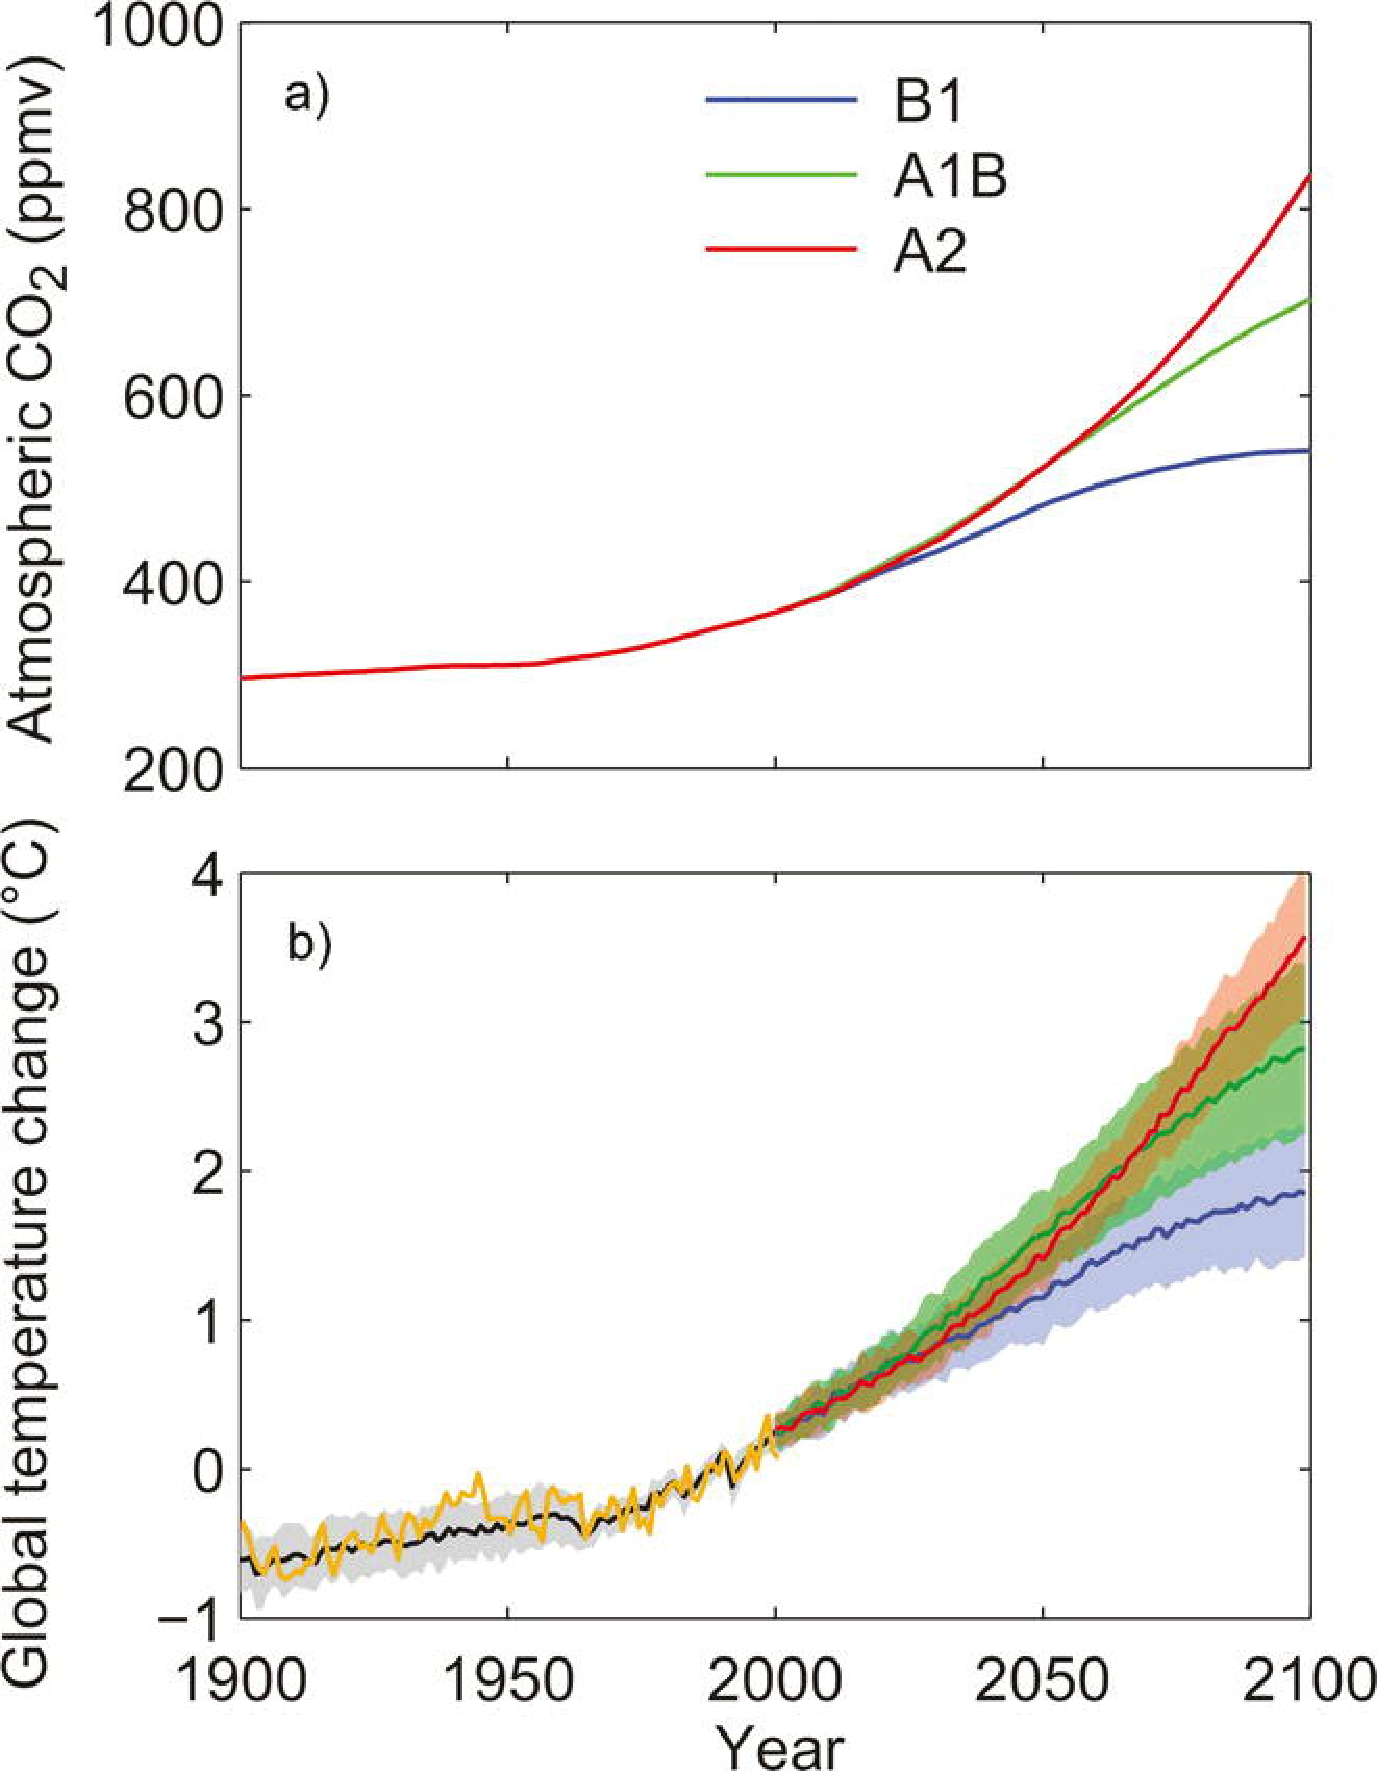
\includegraphics[width=19pc,angle=0]{figure01.pdf}\\
%\appendcaption{A1}{Caption here.}
%\end{figure}
%
% All appendix figures/tables should be placed in order AFTER the main figures/tables, i.e., tables, appendix tables, figures, appendix figures.
%
%%%%%%%%%%%%%%%%%%%%%%%%%%%%%%%%%%%%%%%%%%%%%%%%%%%%%%%%%%%%%%%%%%%%%
% REFERENCES
%%%%%%%%%%%%%%%%%%%%%%%%%%%%%%%%%%%%%%%%%%%%%%%%%%%%%%%%%%%%%%%%%%%%%
% Make your BibTeX bibliography by using these commands:
% \bibliographystyle{ametsoc2014}
% \bibliography{references}

\bibliographystyle{ametsoc2014}
\bibliography{references}

%%%%%%%%%%%%%%%%%%%%%%%%%%%%%%%%%%%%%%%%%%%%%%%%%%%%%%%%%%%%%%%%%%%%%
% TABLES
%%%%%%%%%%%%%%%%%%%%%%%%%%%%%%%%%%%%%%%%%%%%%%%%%%%%%%%%%%%%%%%%%%%%%
%% Enter tables at the end of the document, before figures.
%%
%
%\begin{table}[t]
%\caption{This is a sample table caption and table layout.  Enter as many tables as
%  necessary at the end of your manuscript. Table from Lorenz (1963).}\label{t1}
%\begin{center}
%\begin{tabular}{ccccrrcrc}
%\hline\hline
%$N$ & $X$ & $Y$ & $Z$\\
%\hline
% 0000 & 0000 & 0010 & 0000 \\
% 0005 & 0004 & 0012 & 0000 \\
% 0010 & 0009 & 0020 & 0000 \\
% 0015 & 0016 & 0036 & 0002 \\
% 0020 & 0030 & 0066 & 0007 \\
% 0025 & 0054 & 0115 & 0024 \\
%\hline
%\end{tabular}
%\end{center}
%\end{table}

%%%%%%%%%%%%%%%%%%%%%%%%%%%%%%%%%%%%%%%%%%%%%%%%%%%%%%%%%%%%%%%%%%%%%
% FIGURES
%%%%%%%%%%%%%%%%%%%%%%%%%%%%%%%%%%%%%%%%%%%%%%%%%%%%%%%%%%%%%%%%%%%%%
%% Enter figures at the end of the document, after tables.
%%
%
%\begin{figure}[t]
%  \noindent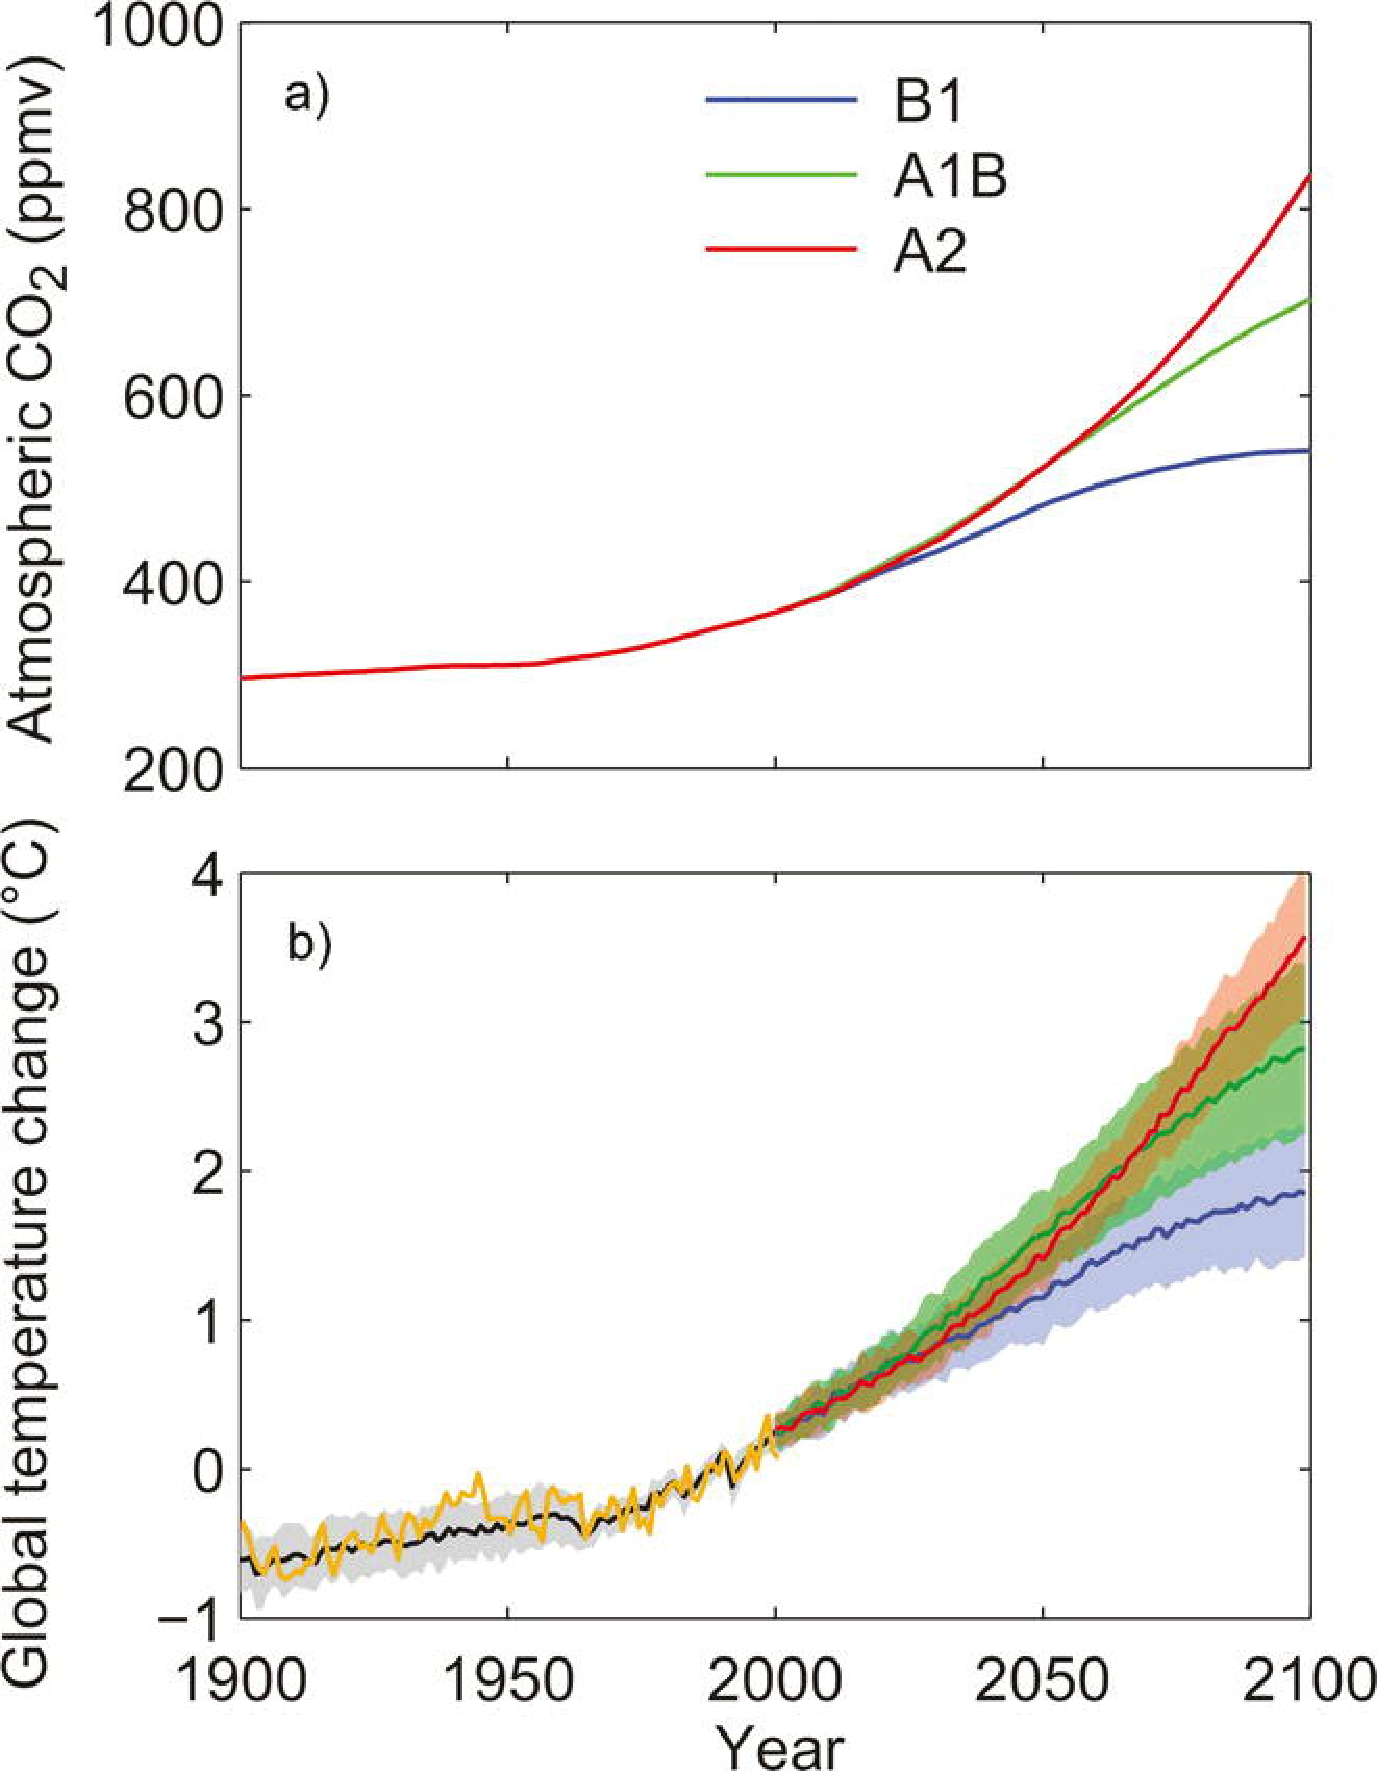
\includegraphics[width=19pc,angle=0]{figure01.pdf}\\
%  \caption{Enter the caption for your figure here.  Repeat as
%  necessary for each of your figures. Figure from \protect\cite{Knutti2008}.}\label{f1}
%\end{figure}

\end{document}